\documentclass[tikz,border=6pt]{standalone}
\usepackage{fontspec}
\usepackage{xeCJK}
\setmainfont{Times New Roman}
\setCJKmainfont{Hiragino Sans GB}
\setCJKsansfont{Microsoft YaHei}
\setCJKmonofont{STSong}
\usepackage{xcolor}
\usetikzlibrary{decorations.pathmorphing}

\definecolor{massblue}{HTML}{4A90D9}
\definecolor{linegray}{HTML}{333333}

\begin{document}
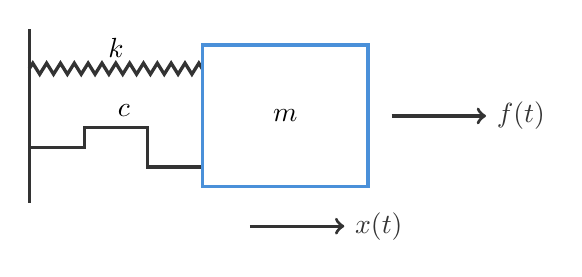
\begin{tikzpicture}[line width=1.2pt]
  \draw[linegray] (0,0) -- (0,2.2);
  \draw[linegray, decorate, decoration={zigzag, segment length=5pt, amplitude=2pt}] (0,1.7) -- (2.2,1.7);
  \draw[linegray] (0,0.7) -- (0.7,0.7) -- (0.7,0.95) -- (1.5,0.95) -- (1.5,0.45) -- (2.2,0.45);
  \draw[massblue] (2.2,0.2) rectangle (4.3,2.0);
  \node at (3.25,1.1) {$m$};
  \node[above] at (1.1,1.7) {$k$};
  \node[above] at (1.2,0.95) {$c$};
  \draw[linegray, ->] (4.6,1.1) -- (5.8,1.1) node[right] {$f(t)$};
  \draw[linegray, ->] (2.8,-0.3) -- (4.0,-0.3) node[right] {$x(t)$};
\end{tikzpicture}
\end{document}
